% ------------------------------------------------------------------------ %
% !TEX encoding = UTF-8
% !TEX TS-program = pdflatex
% !TEX root = ../Project.tex
% !TEX spellcheck = en-EN
% ------------------------------------------------------------------------ %
%
% ------------------------------------------------------------------------ %
% 	CHAPTER TITLE
% ------------------------------------------------------------------------ %
%
\chapter{Design-in-the-small}
%
The fixed elements in every page are the banner at the top of every page (containing the Help us landmark), the landmarks, that we decided to divide into two groups: one of landmarks regarding exposing content and the other of the landmarks answering more practical questions; and in the end the breadcrumb for orientation info, which is in every page except the homepage. In the homepage we decided to put a big image slideshow presenting the three groups of locations, people and services, because they are the main component of the association. Under that we selected three topics corredated with a description which, in our opinion, are the more useful for a user. The main concept of our site is that pages must be scrolled to see the content, as in most modern websites and applications. The services group page will have a slider to choose between all services and the services grouped by every location, in this way the user will not lose the cognitive space he is in. The other important orientation info is inside every group: there will be a bar telling the user what group is he inside, accompanied by next and previous group link's button to cycle through the other elements of the group. Lastly pages of a topic related to another one contain a list of transition links to the elements of the other topic and, by clicking one of them, the new page will show a description of the group of pages defined by that relation in the orientation info between the next and previous buttons (e.g. From a location page I click one service hosted there, the orientation info of the service will say: "Services hosted in that location" to say that you can cycle through them).
%
\begin{figure}[h]
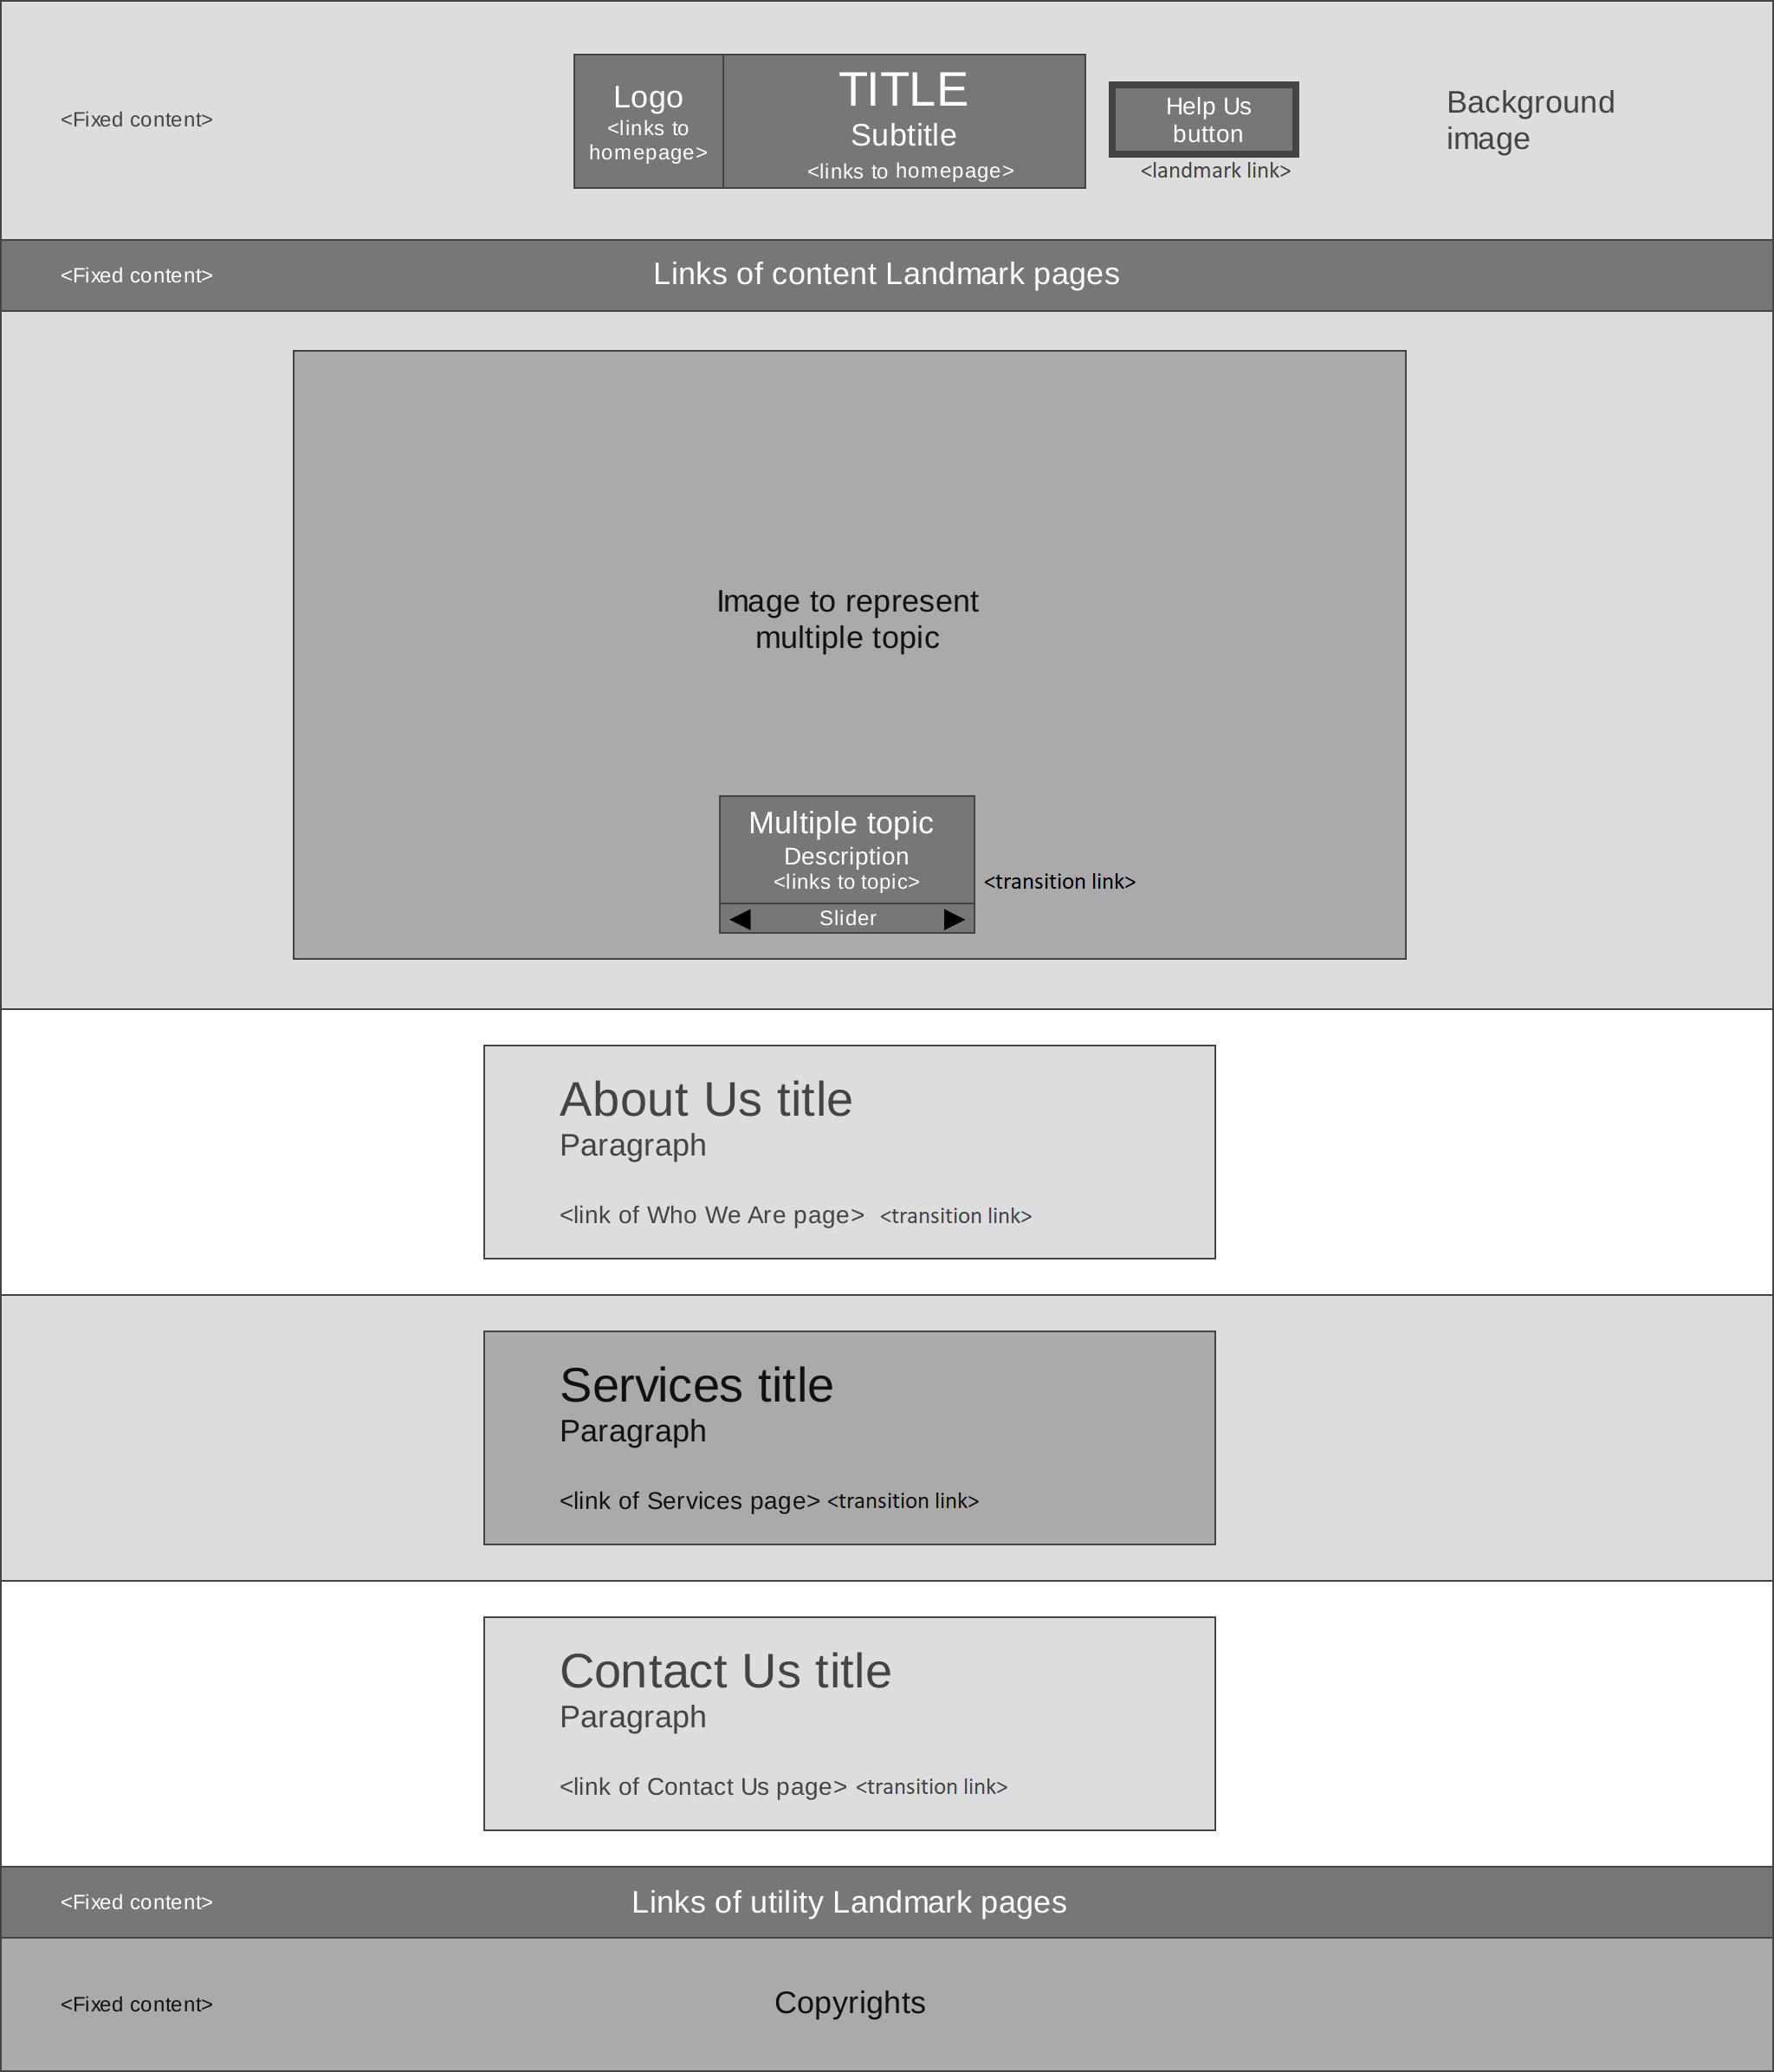
\includegraphics[width=1.27\textwidth, center]{MainMatter/images/1-Homepage}
\caption{Homepage}
\label{fig:figure2}
\end{figure}
%
\begin{figure}[h]
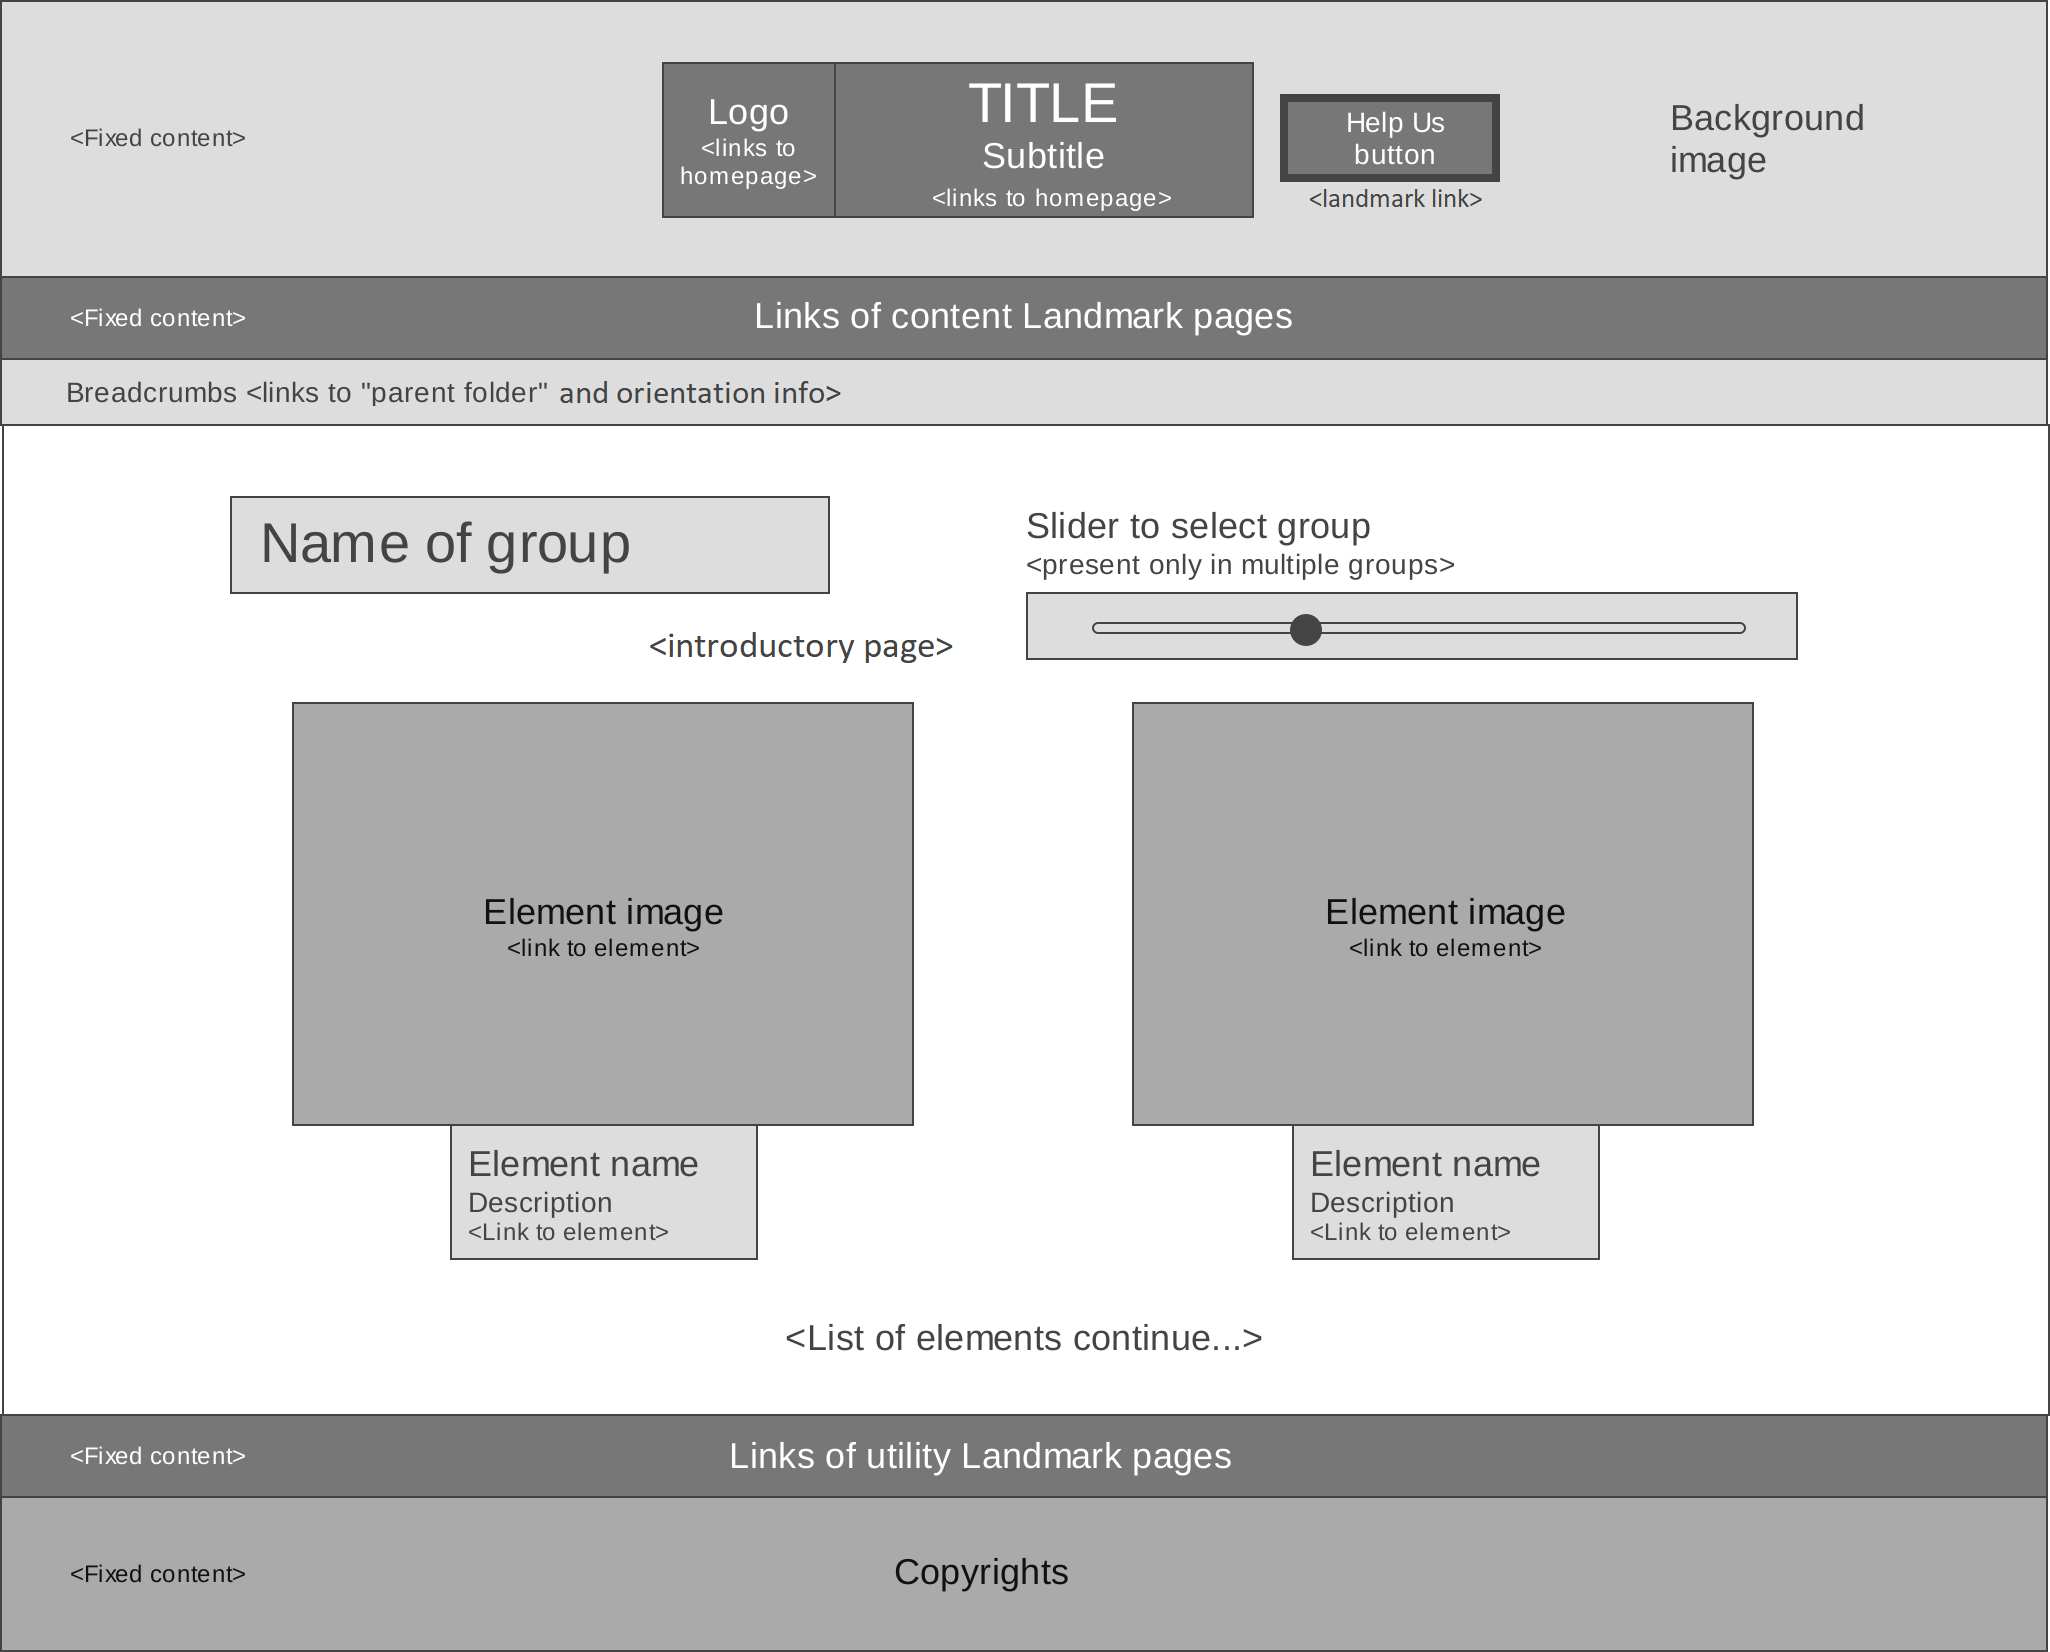
\includegraphics[width=1.3\textwidth, center]{MainMatter/images/2-Group-page}
\caption{People, Services and Locations Group page}
\label{fig:figure2}
\end{figure}
%
\begin{figure}[h]
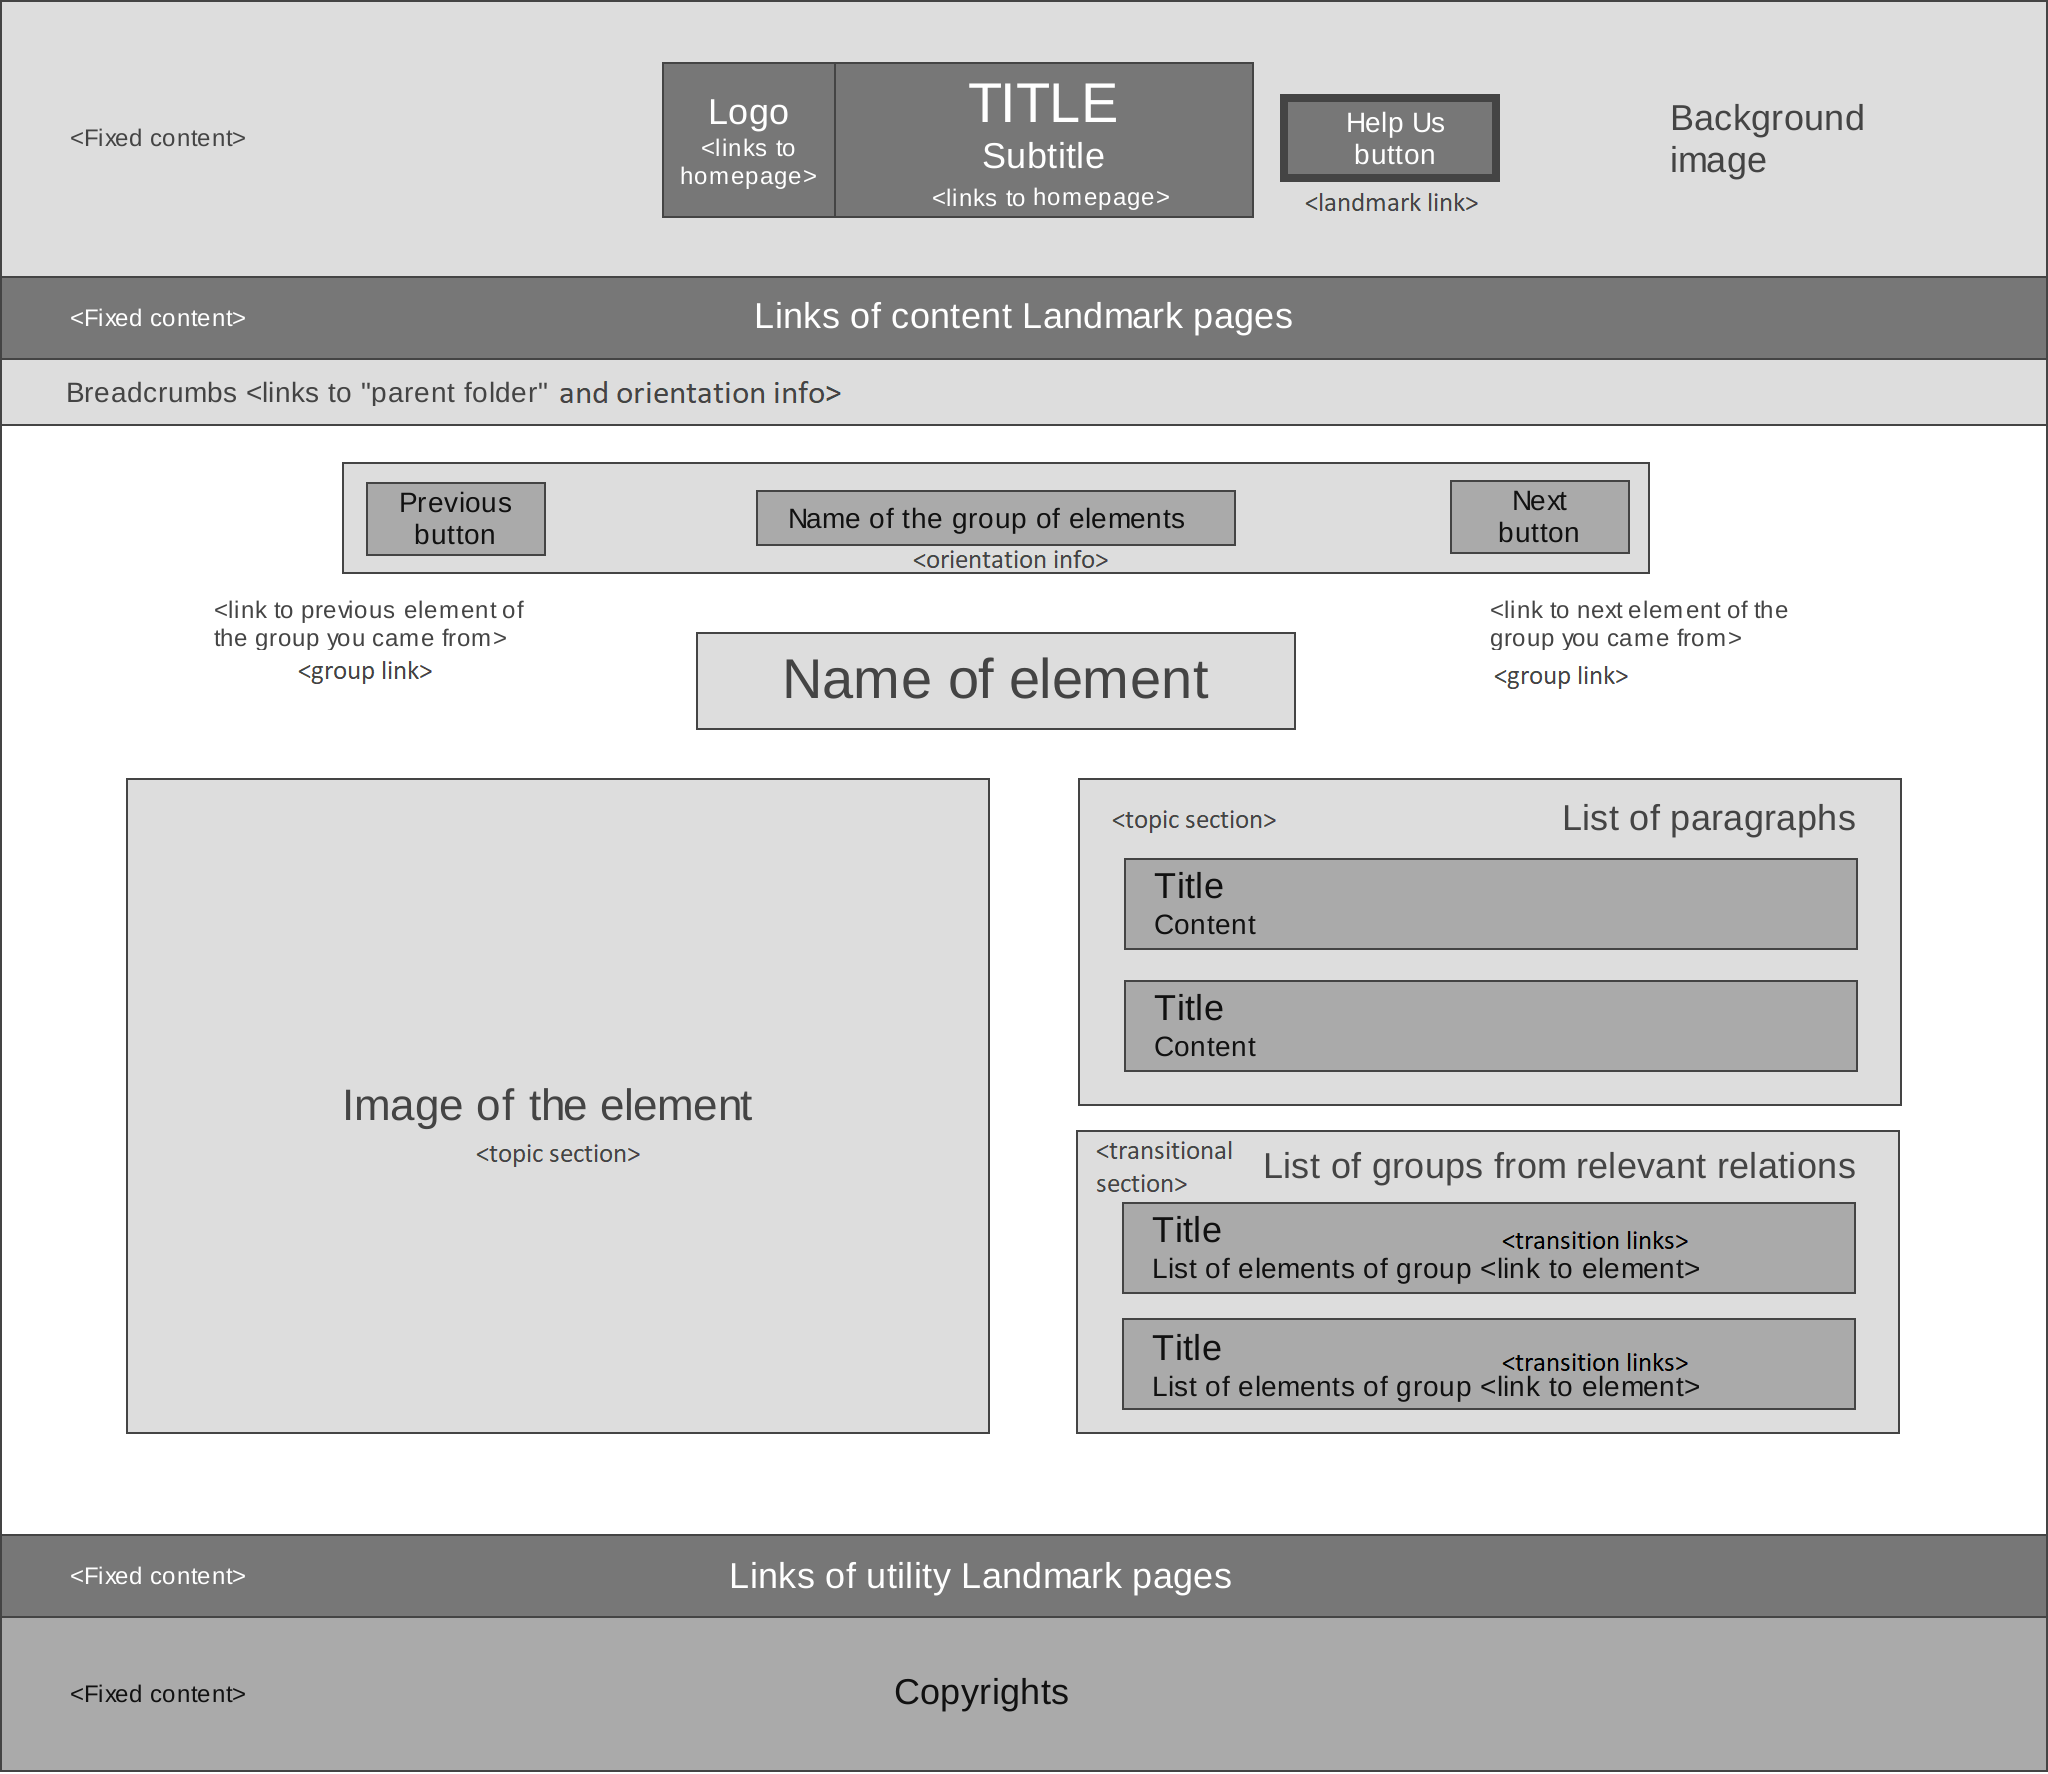
\includegraphics[width=1.3\textwidth, center]{MainMatter/images/3-Multiple-topic-page}
\caption{Person, Service and Location Multiple Topic Page}
\label{fig:figure2}
\end{figure}
%
\begin{figure}[h]
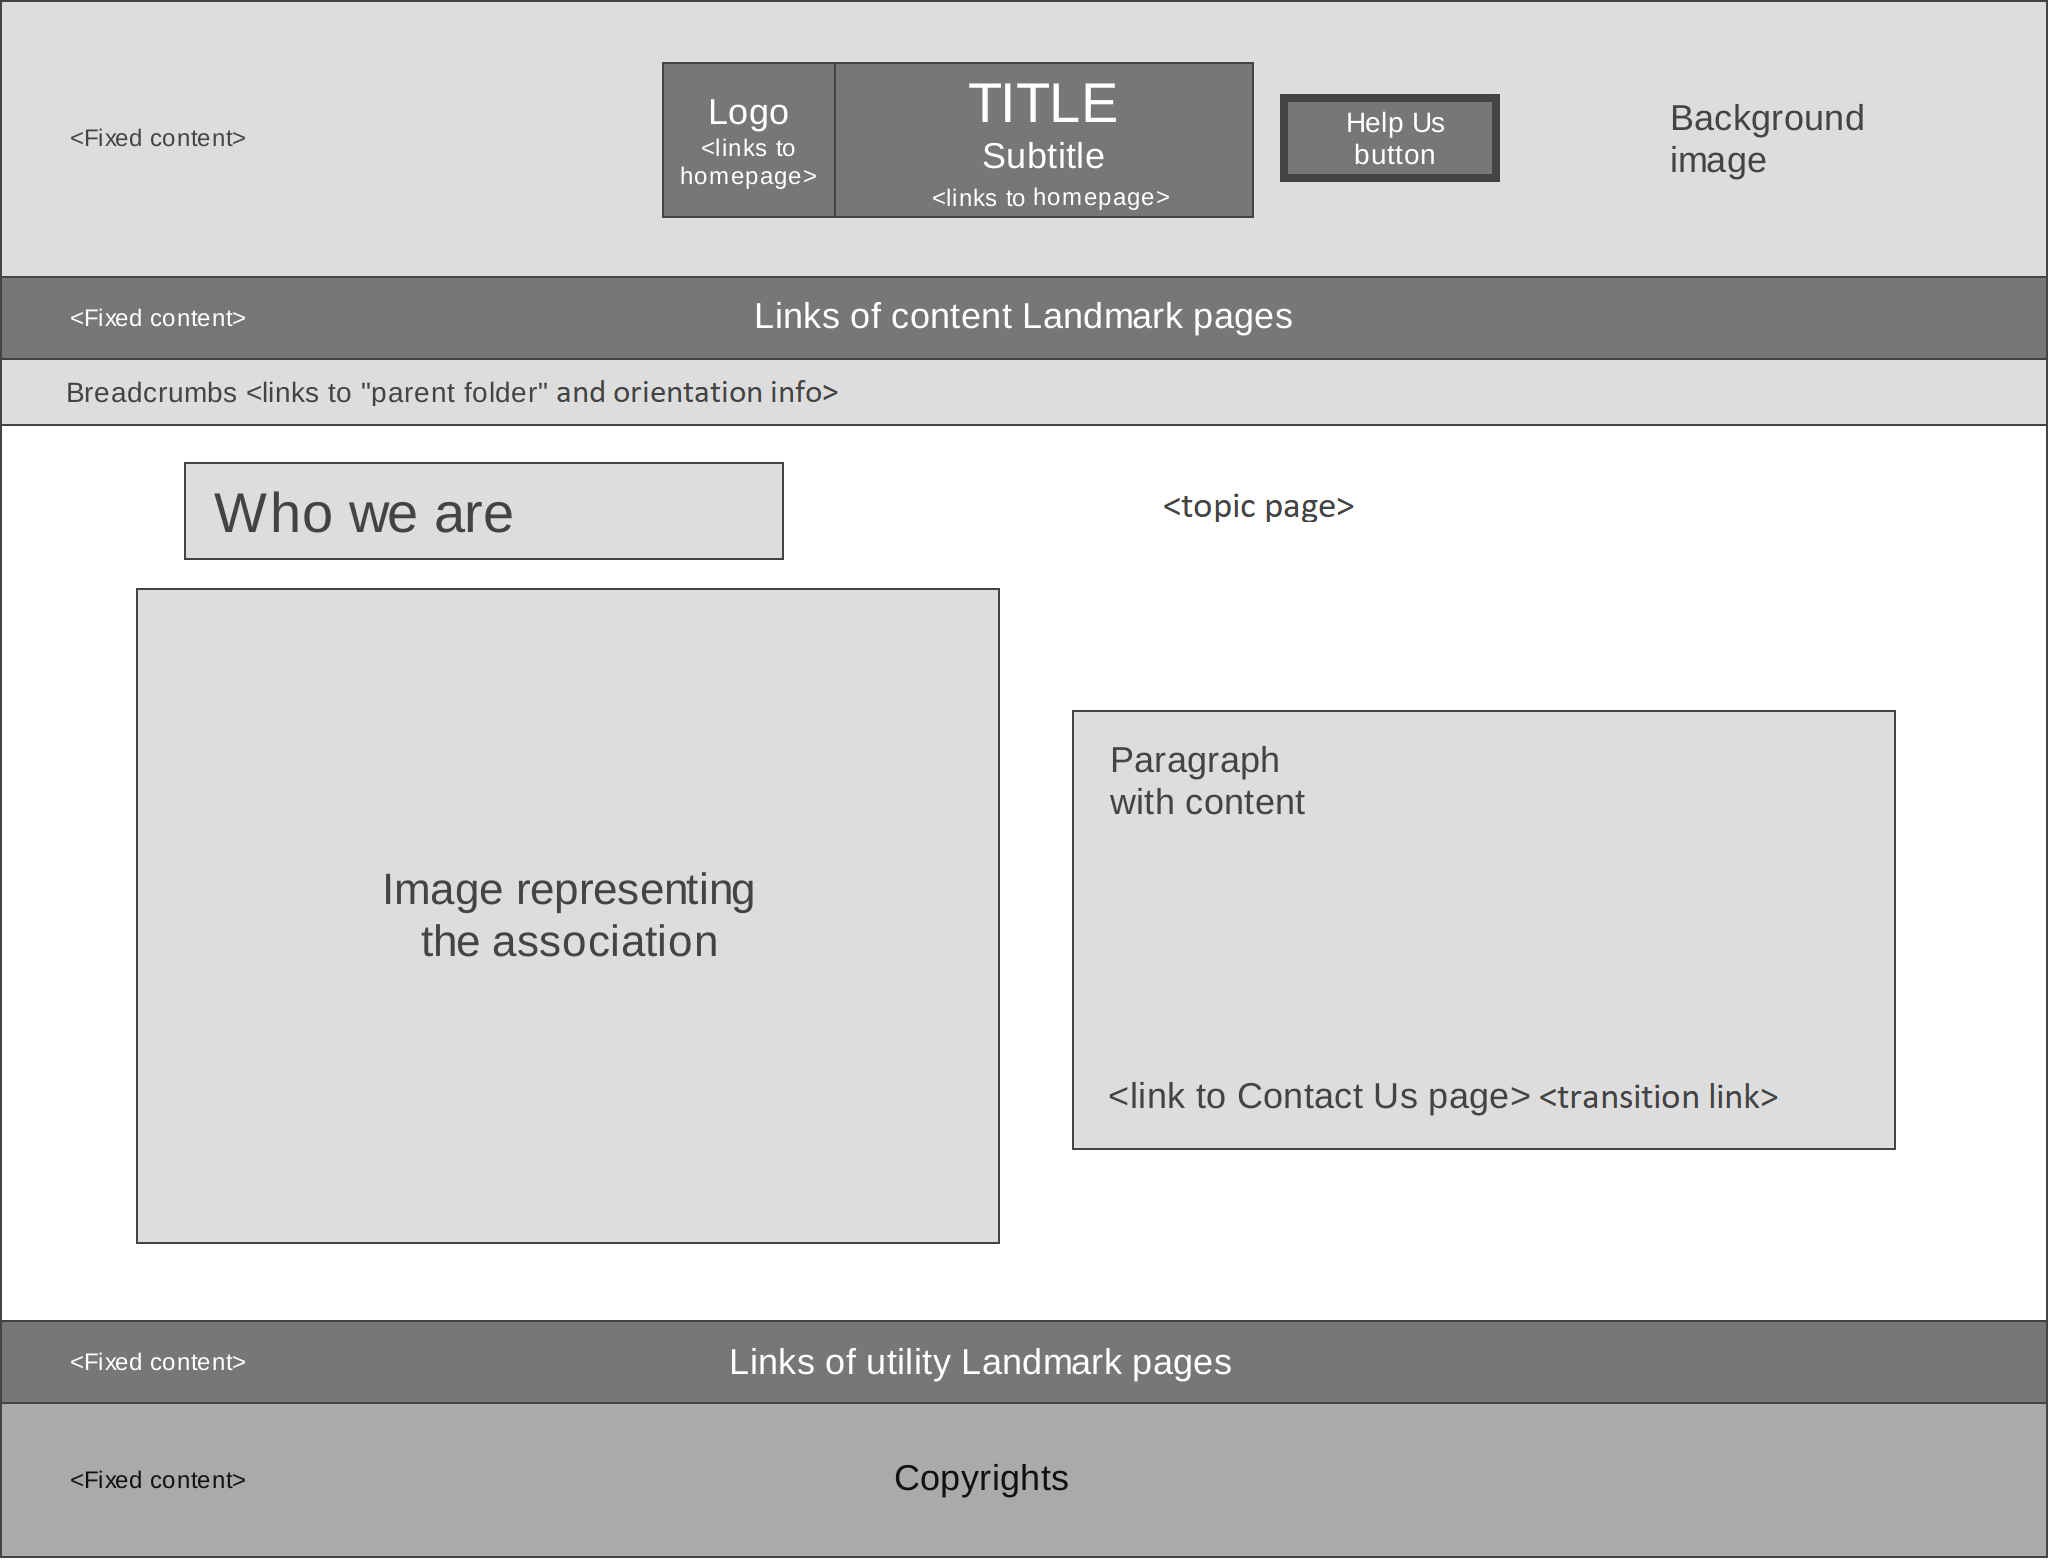
\includegraphics[width=1.3\textwidth, center]{MainMatter/images/4-Single-topic-who-we-are}
\caption{Single topic page: Who we are}
\label{fig:figure2}
\end{figure}
%
\begin{figure}[h]
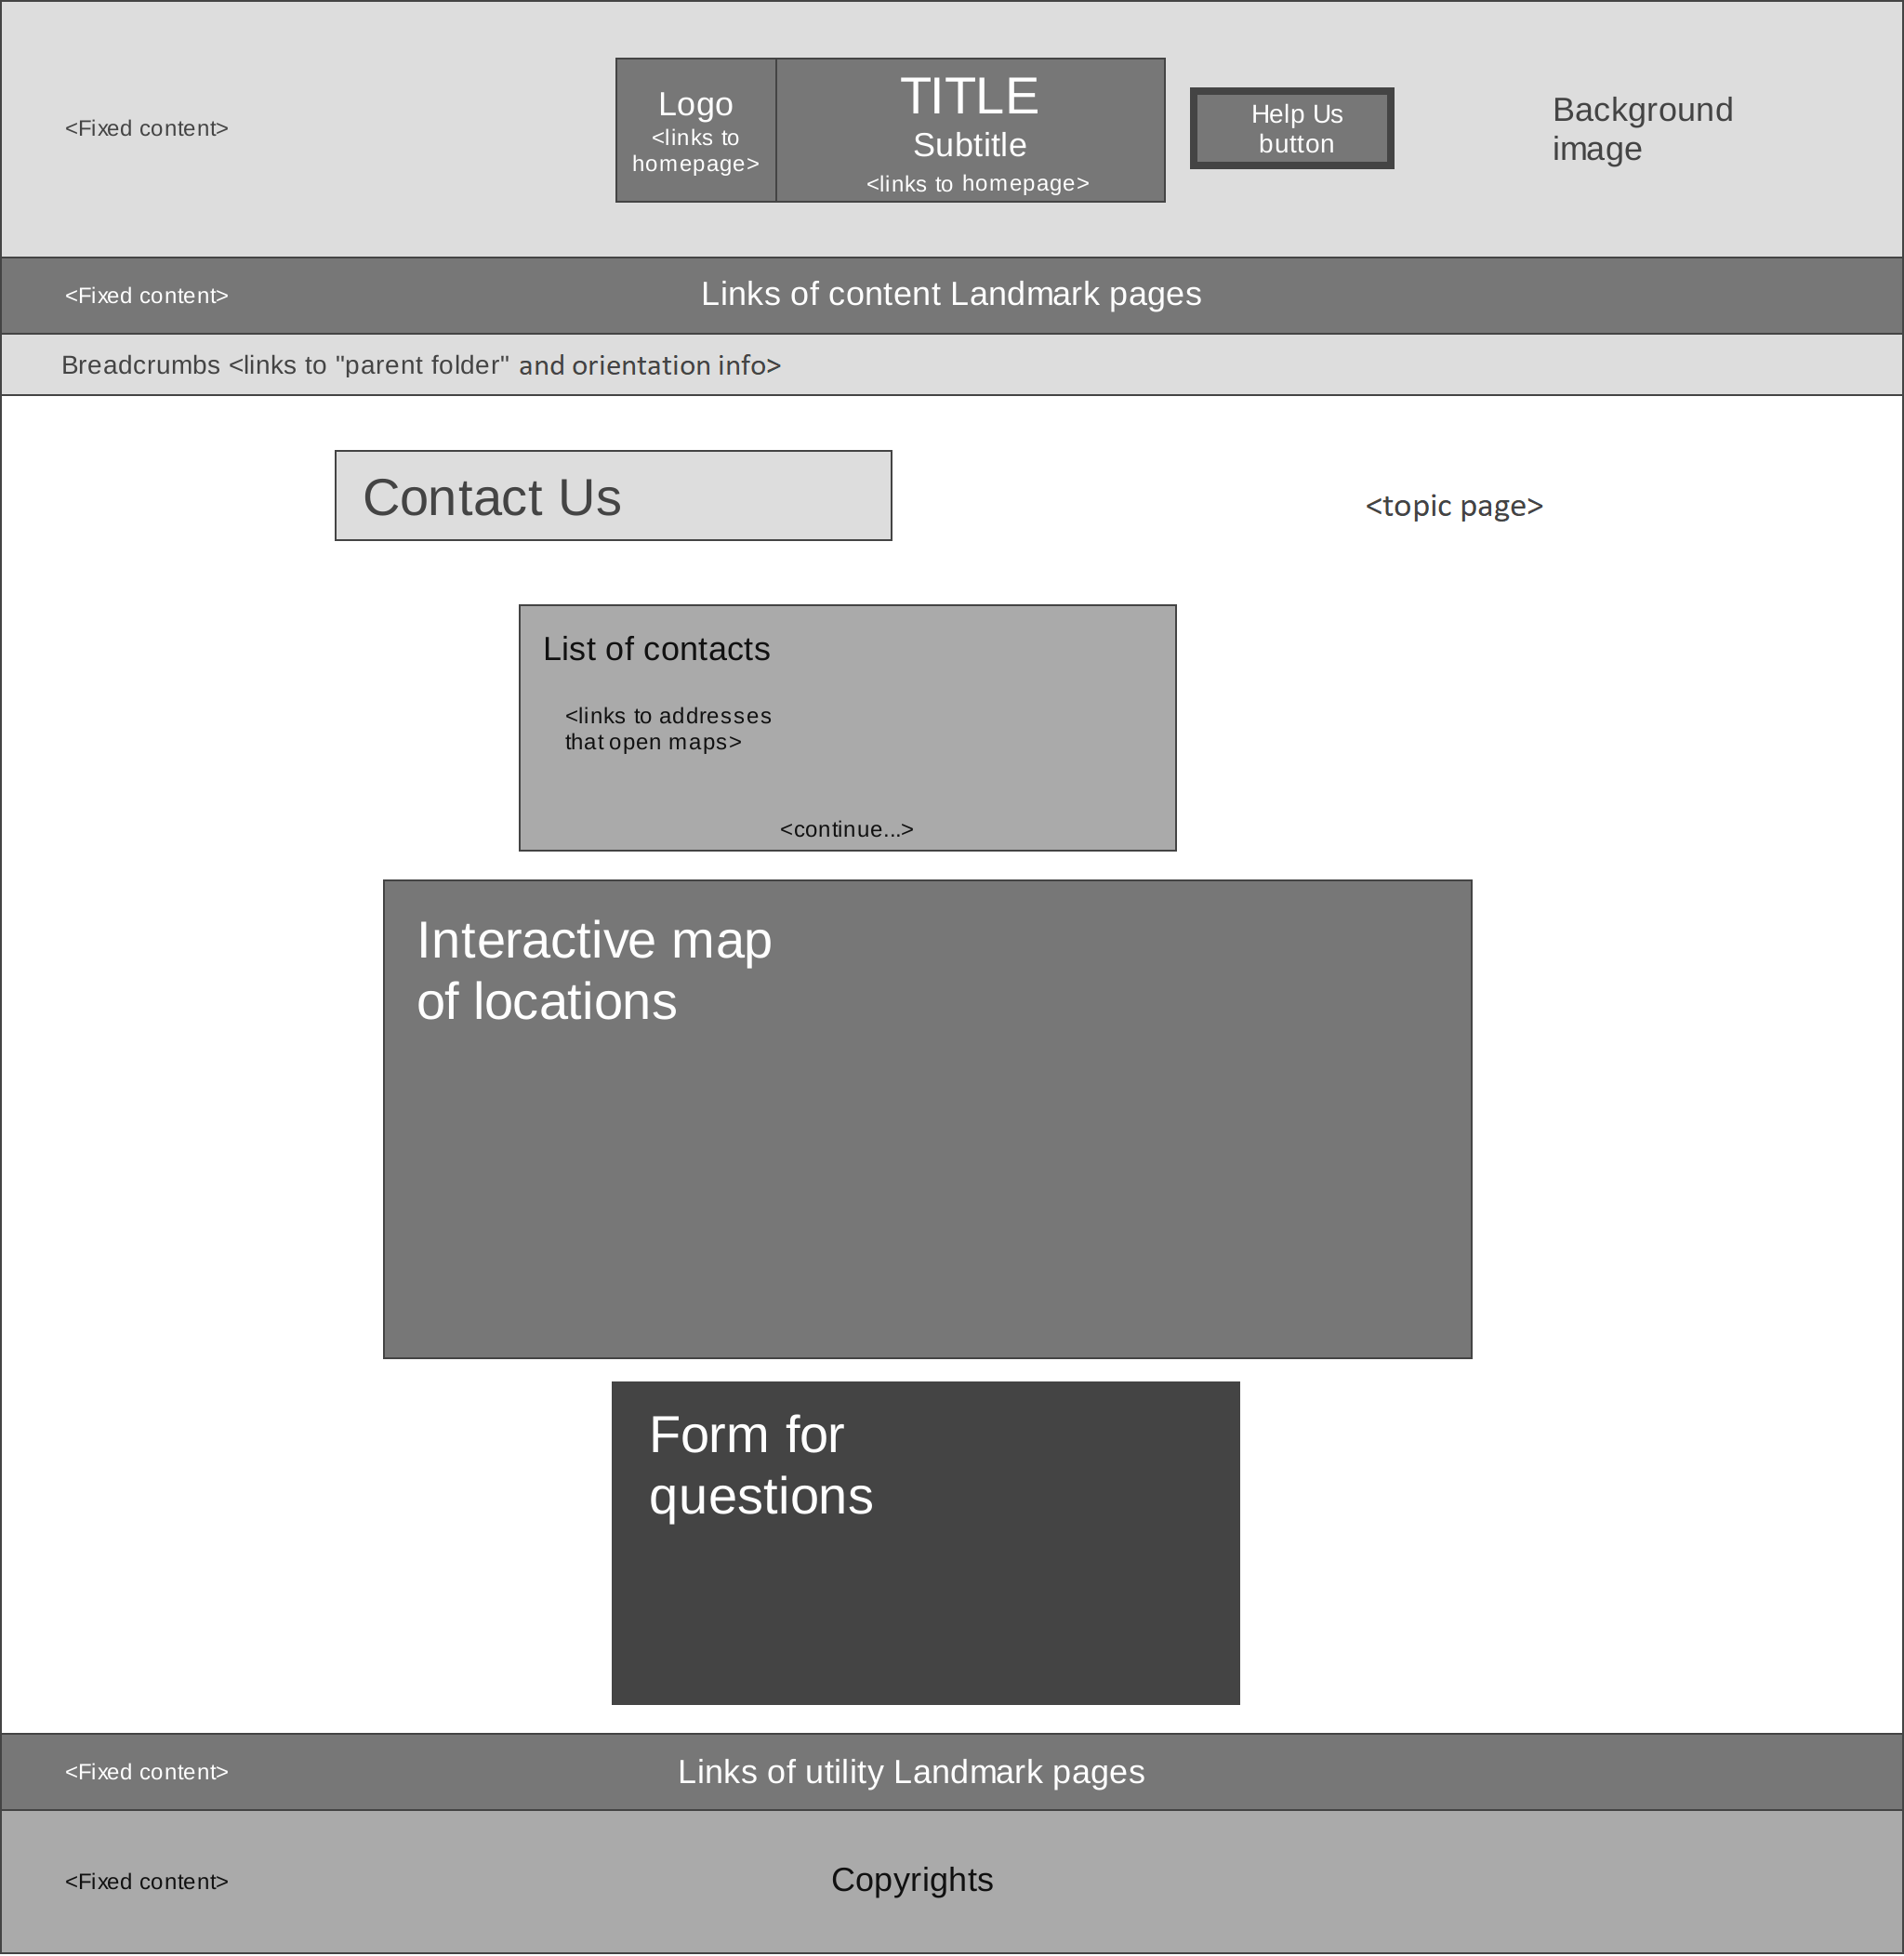
\includegraphics[width=1.3\textwidth, center]{MainMatter/images/5-Single-topic-contact-us}
\caption{Single topic page: Contact us}
\label{fig:figure2}
\end{figure}
%
\begin{figure}[h]
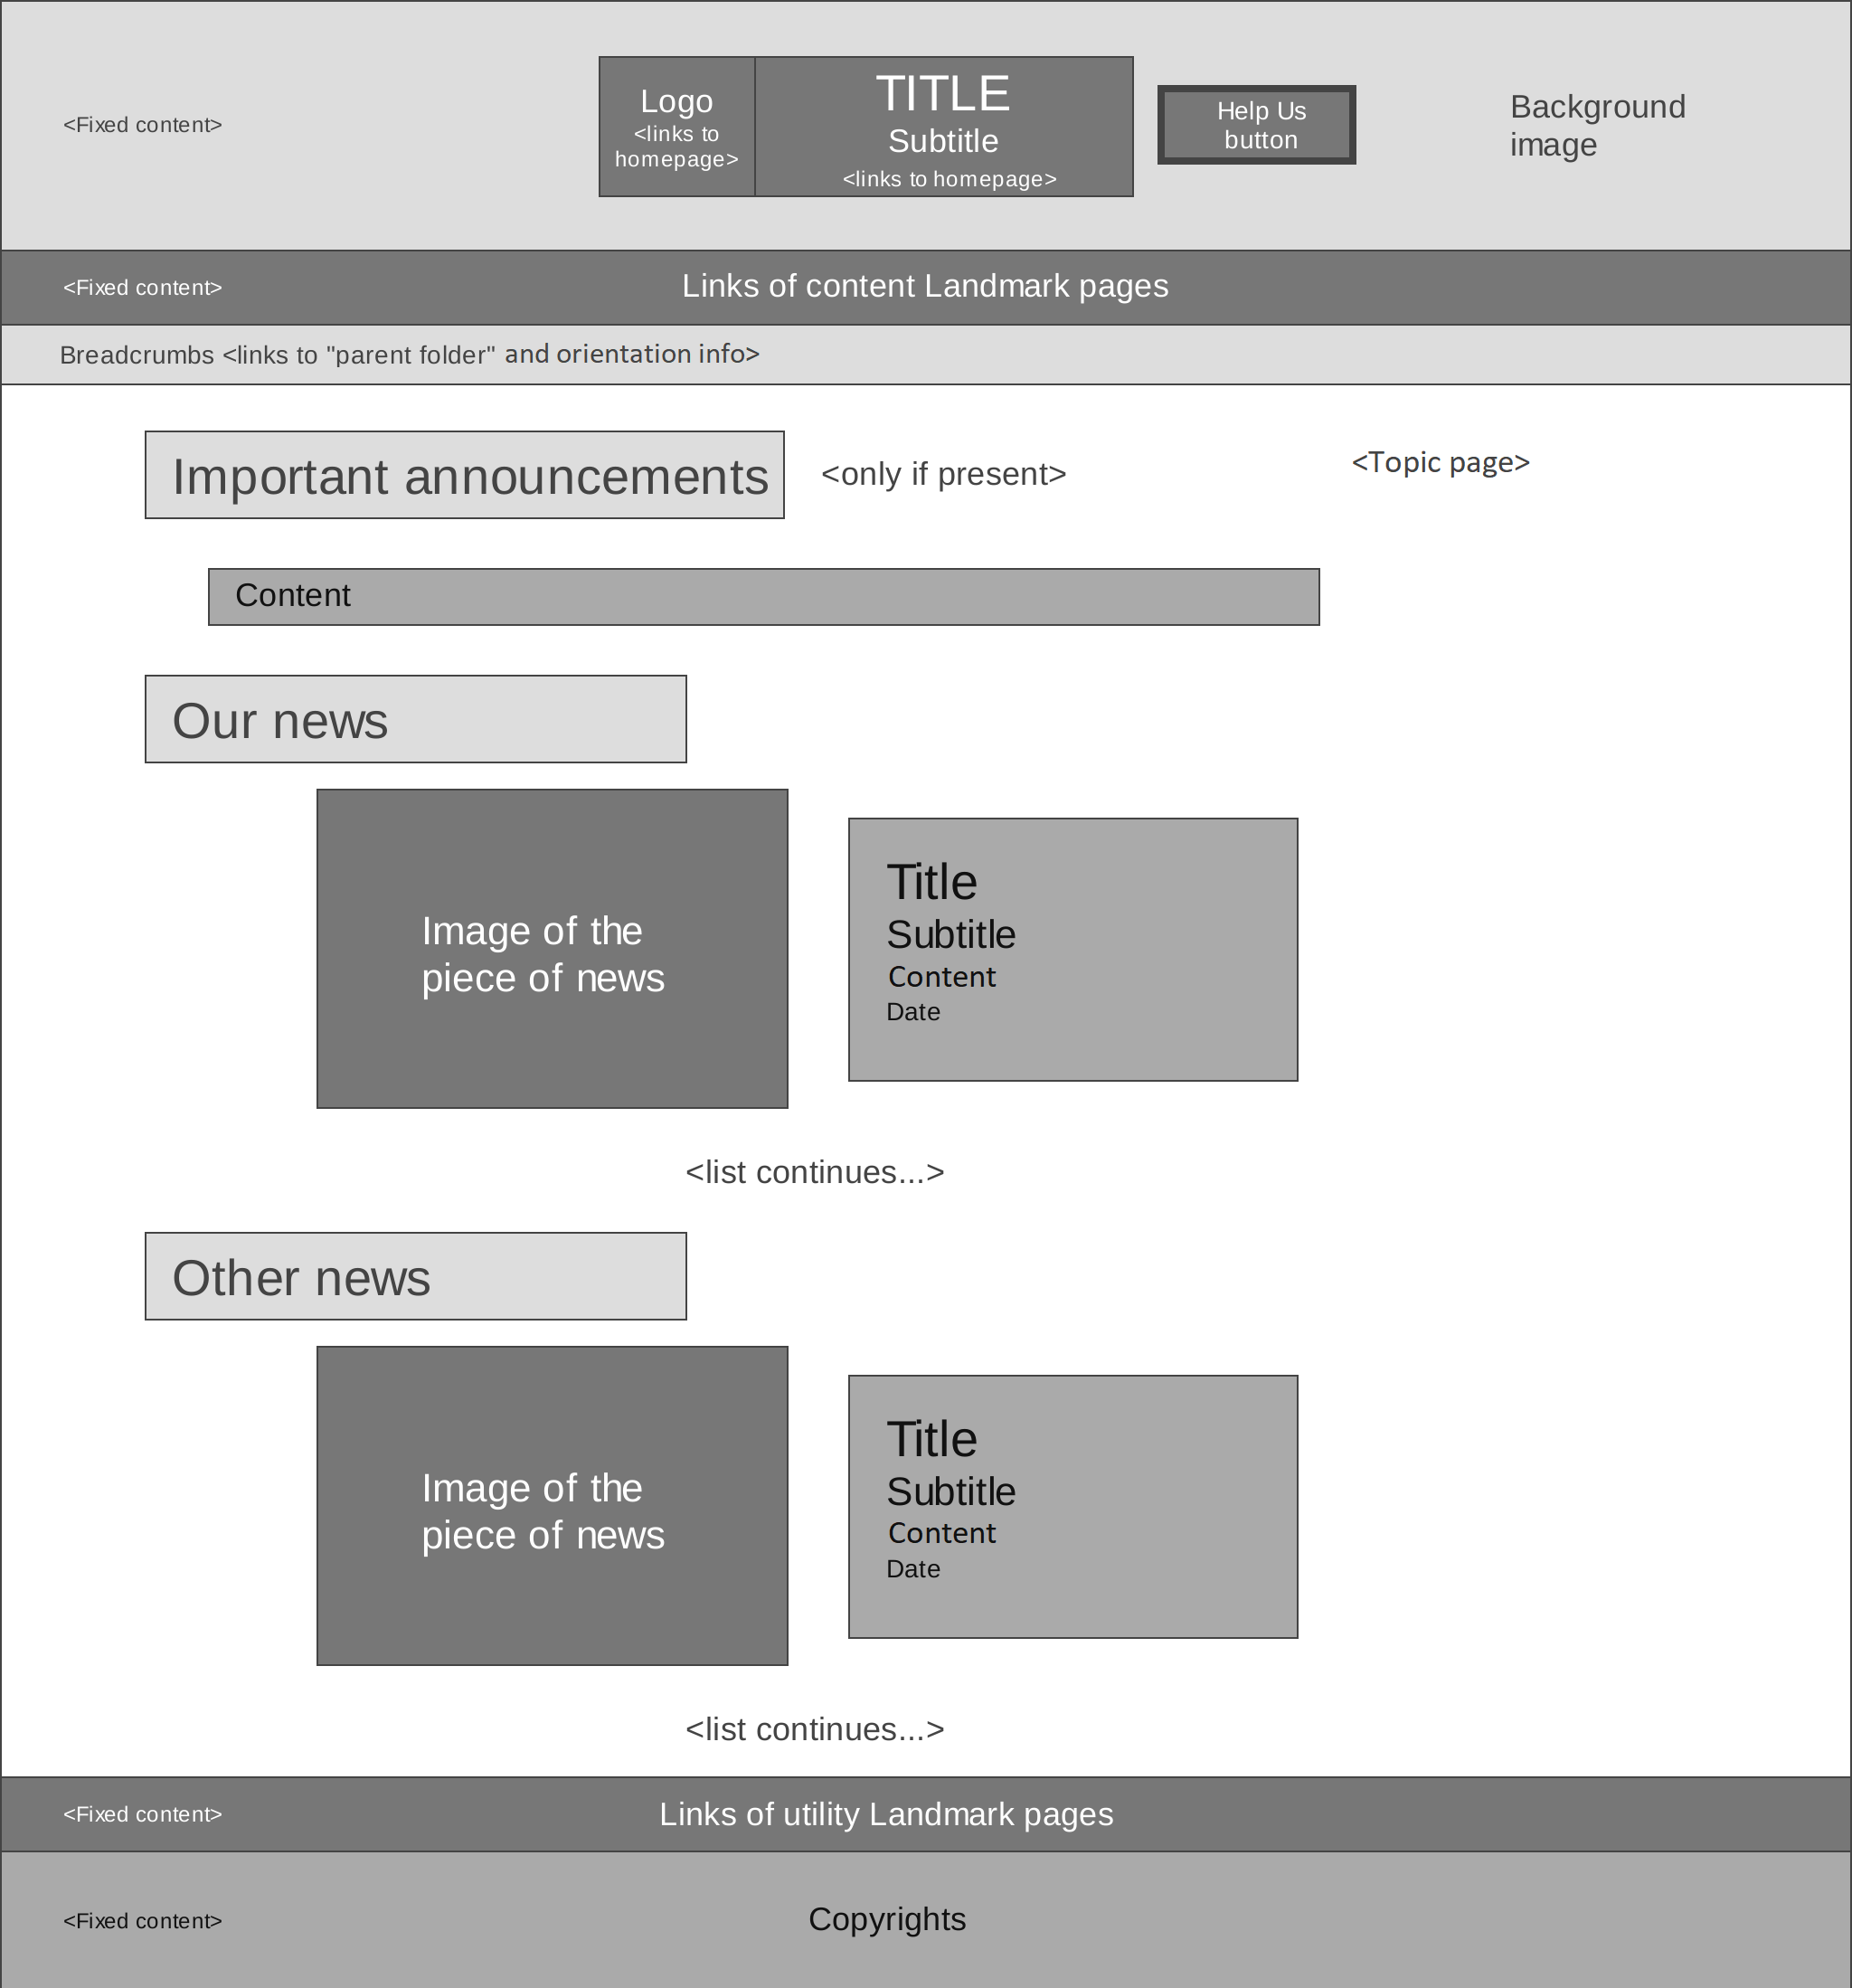
\includegraphics[width=1.3\textwidth, center]{MainMatter/images/6-Single-topic-news}
\caption{Single topic page: News}
\label{fig:figure2}
\end{figure}
%
\begin{figure}[h]
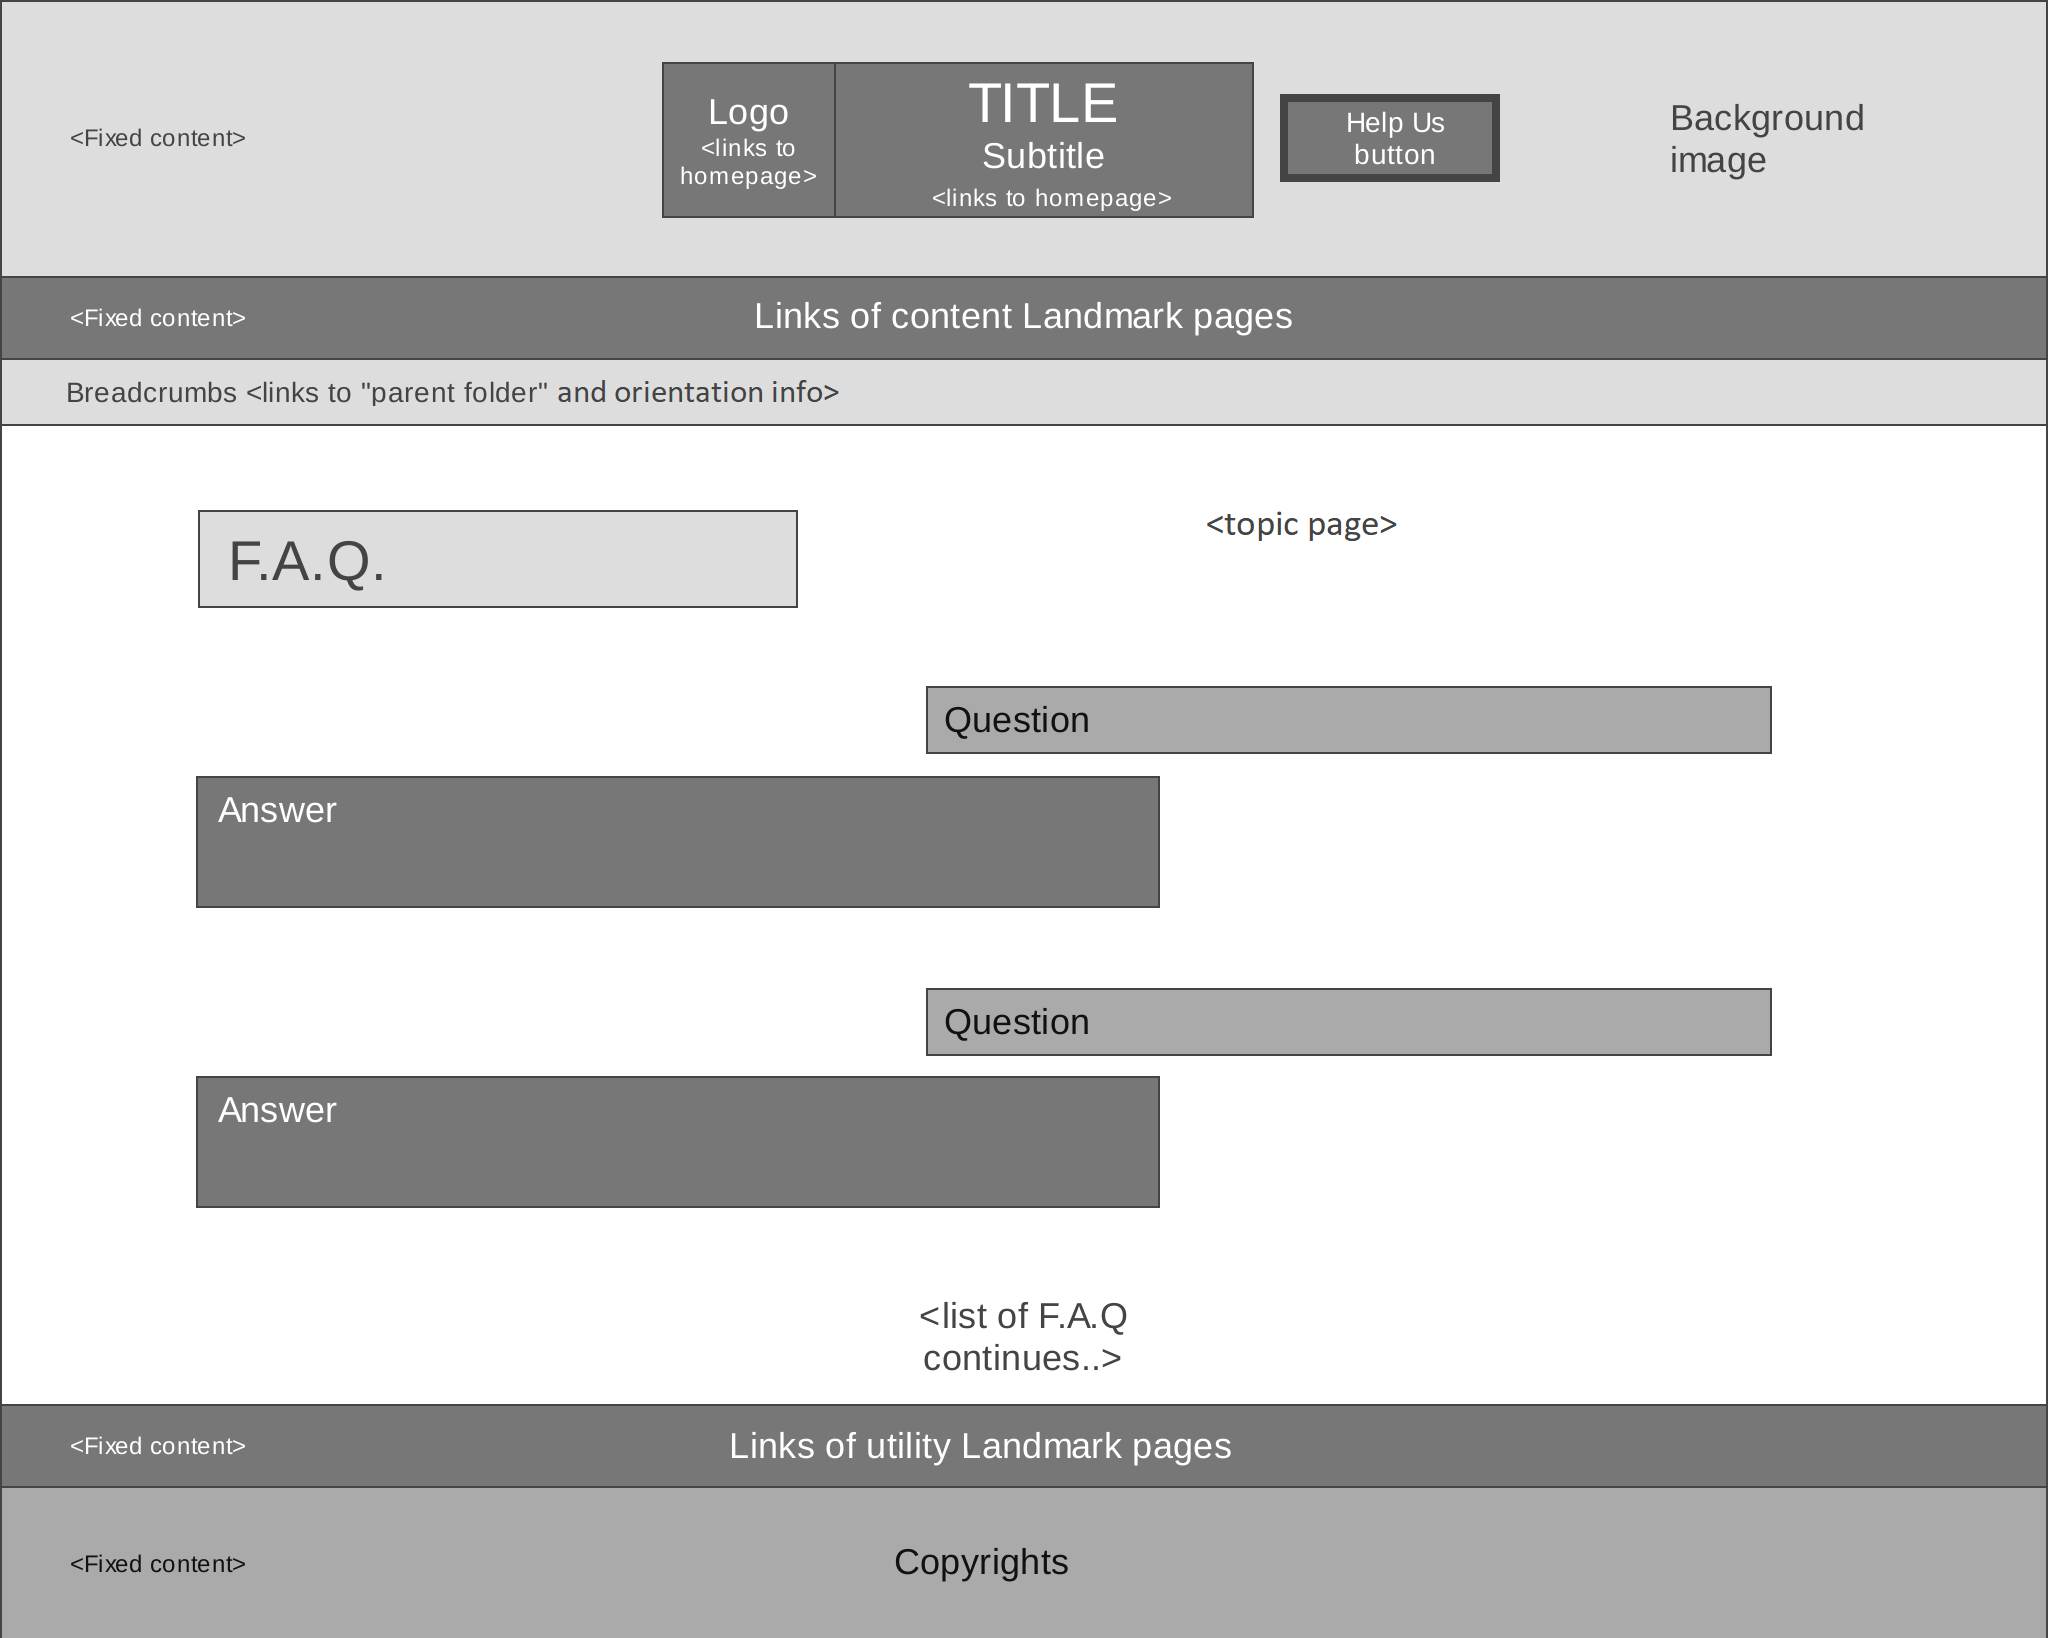
\includegraphics[width=1.3\textwidth, center]{MainMatter/images/7-Single-topic-FAQ}
\caption{Single topic page: F.A.Q.}
\label{fig:figure2}
\end{figure}
%
\begin{figure}[h]
\includegraphics[width=1.3\textwidth, center]{MainMatter/images/8-Group-event}
\caption{Events Group page}
\label{fig:figure2}
\end{figure}
%
\begin{figure}[h]
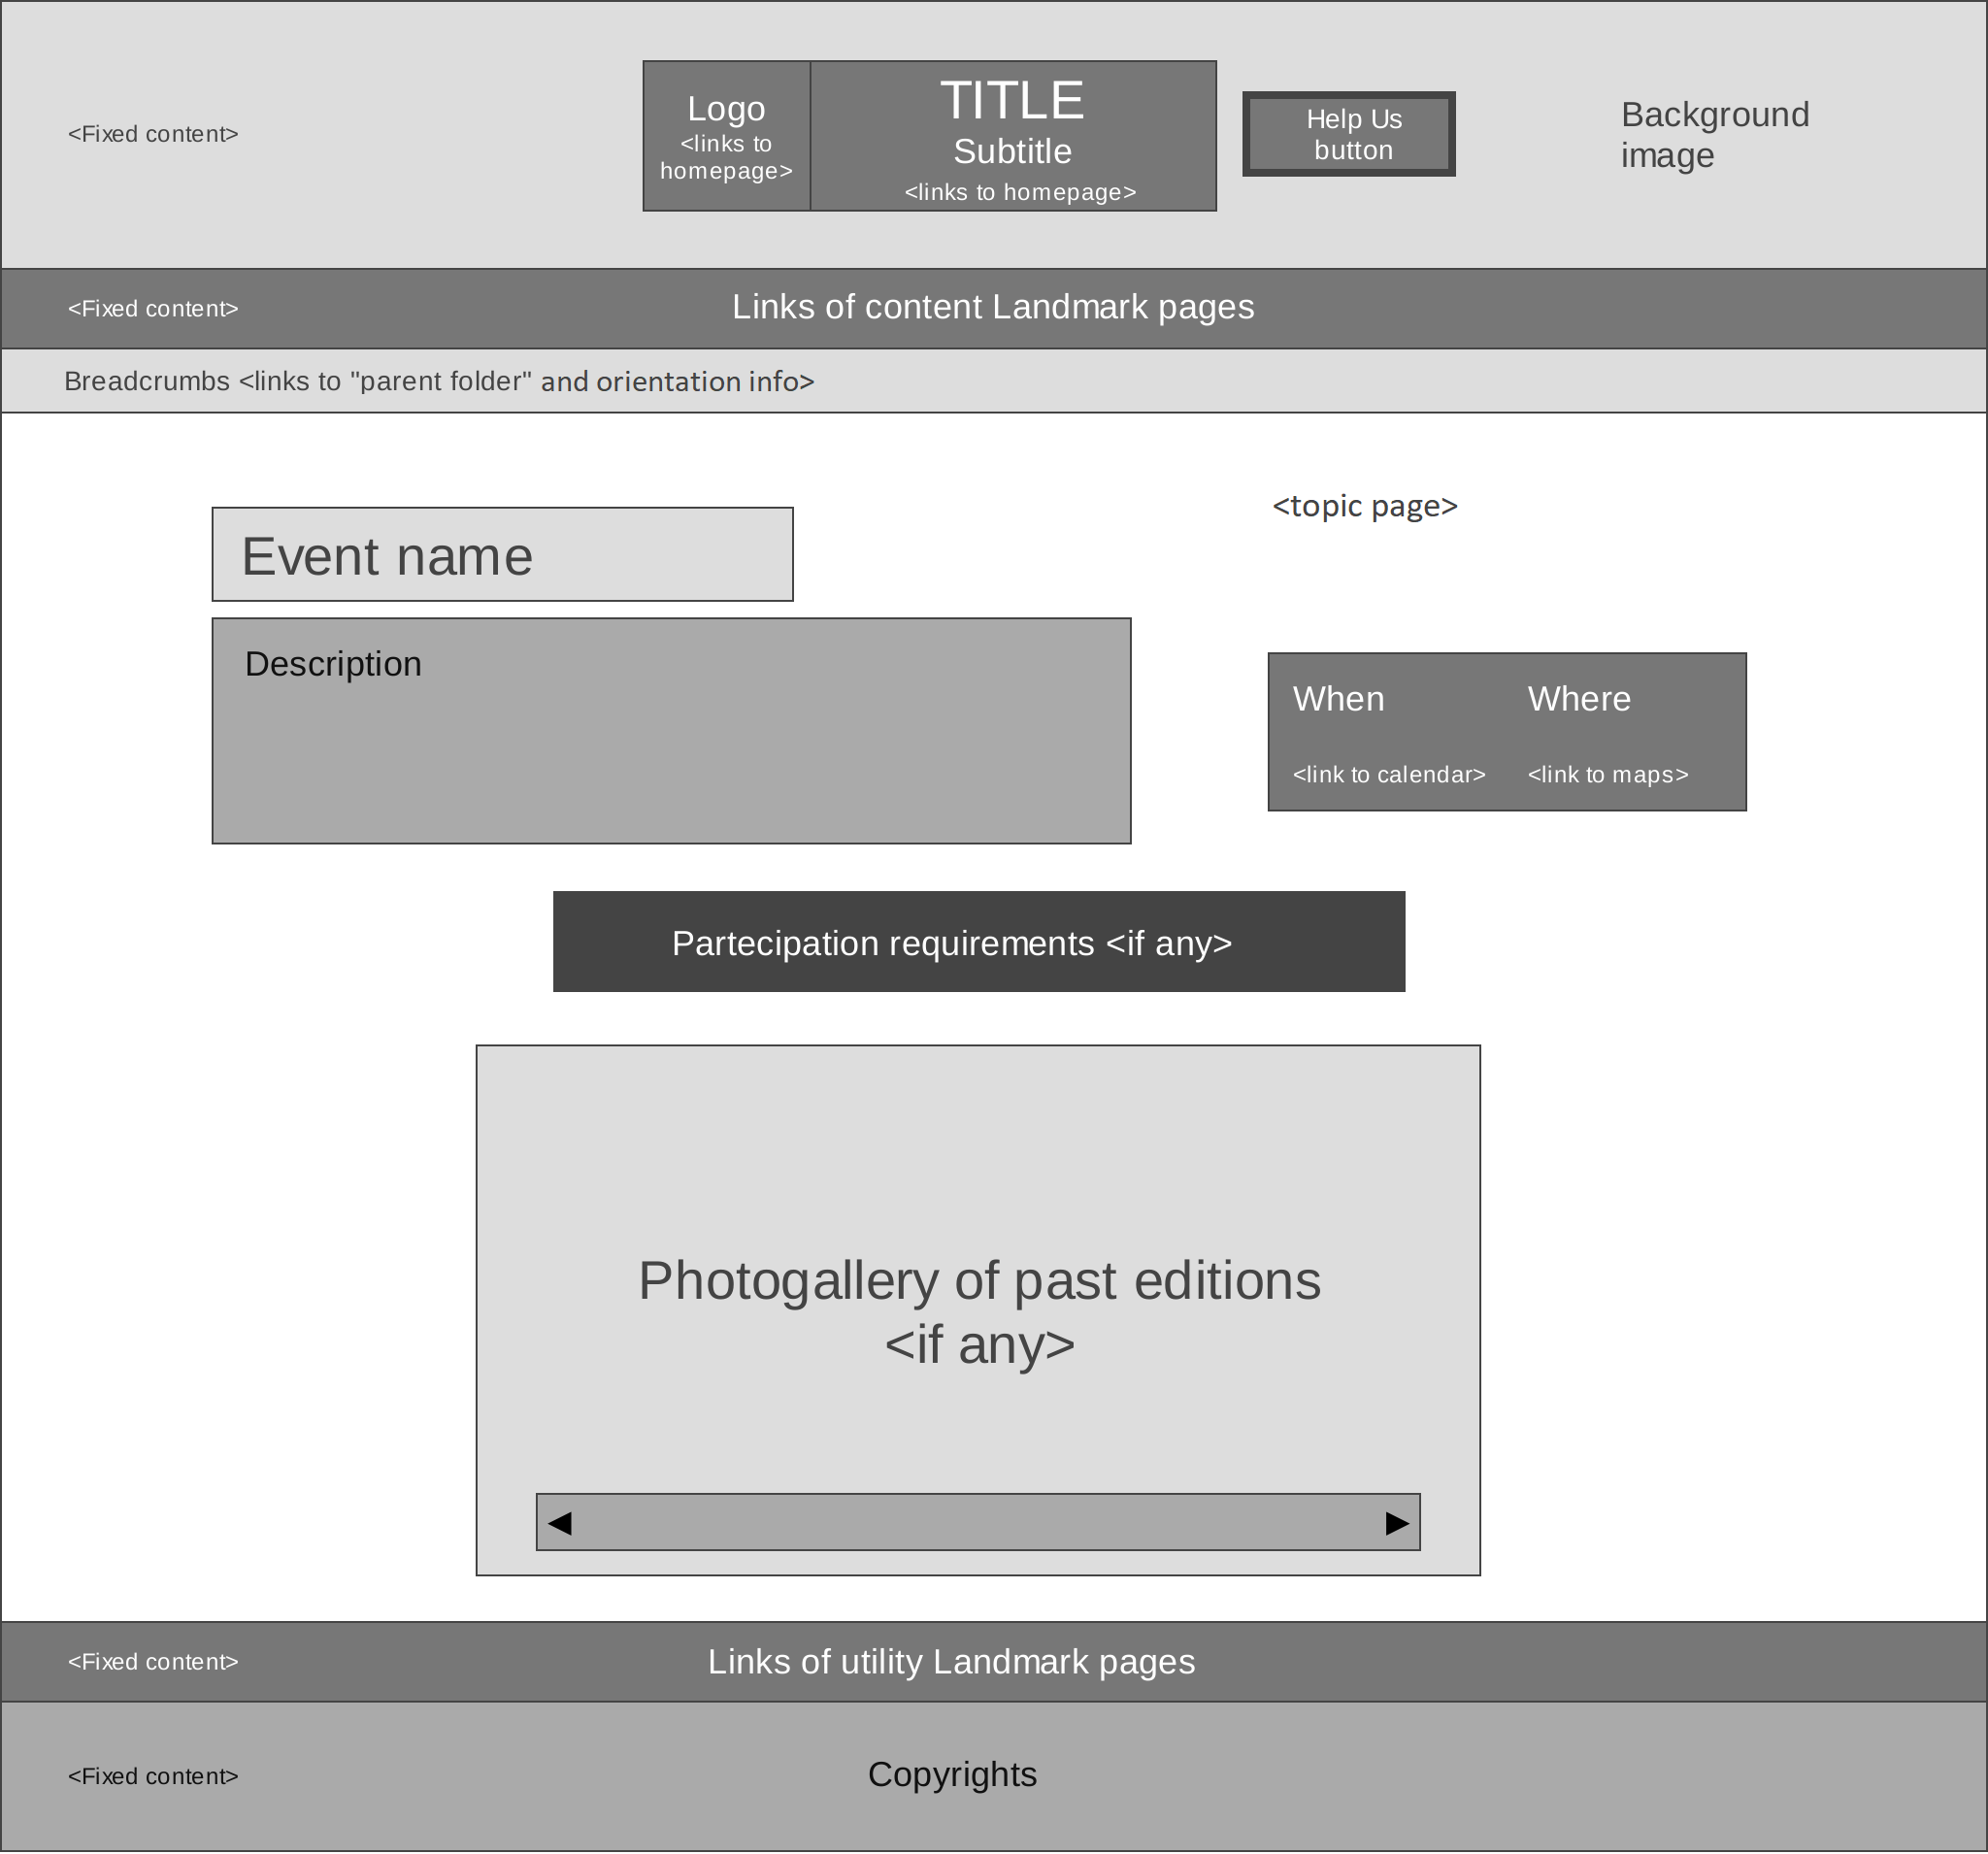
\includegraphics[width=1.3\textwidth, center]{MainMatter/images/9-Multiple-topic-Event}
\caption{Event Multiple Topic Page}
\label{fig:figure2}
\end{figure}
%
\begin{figure}[h]
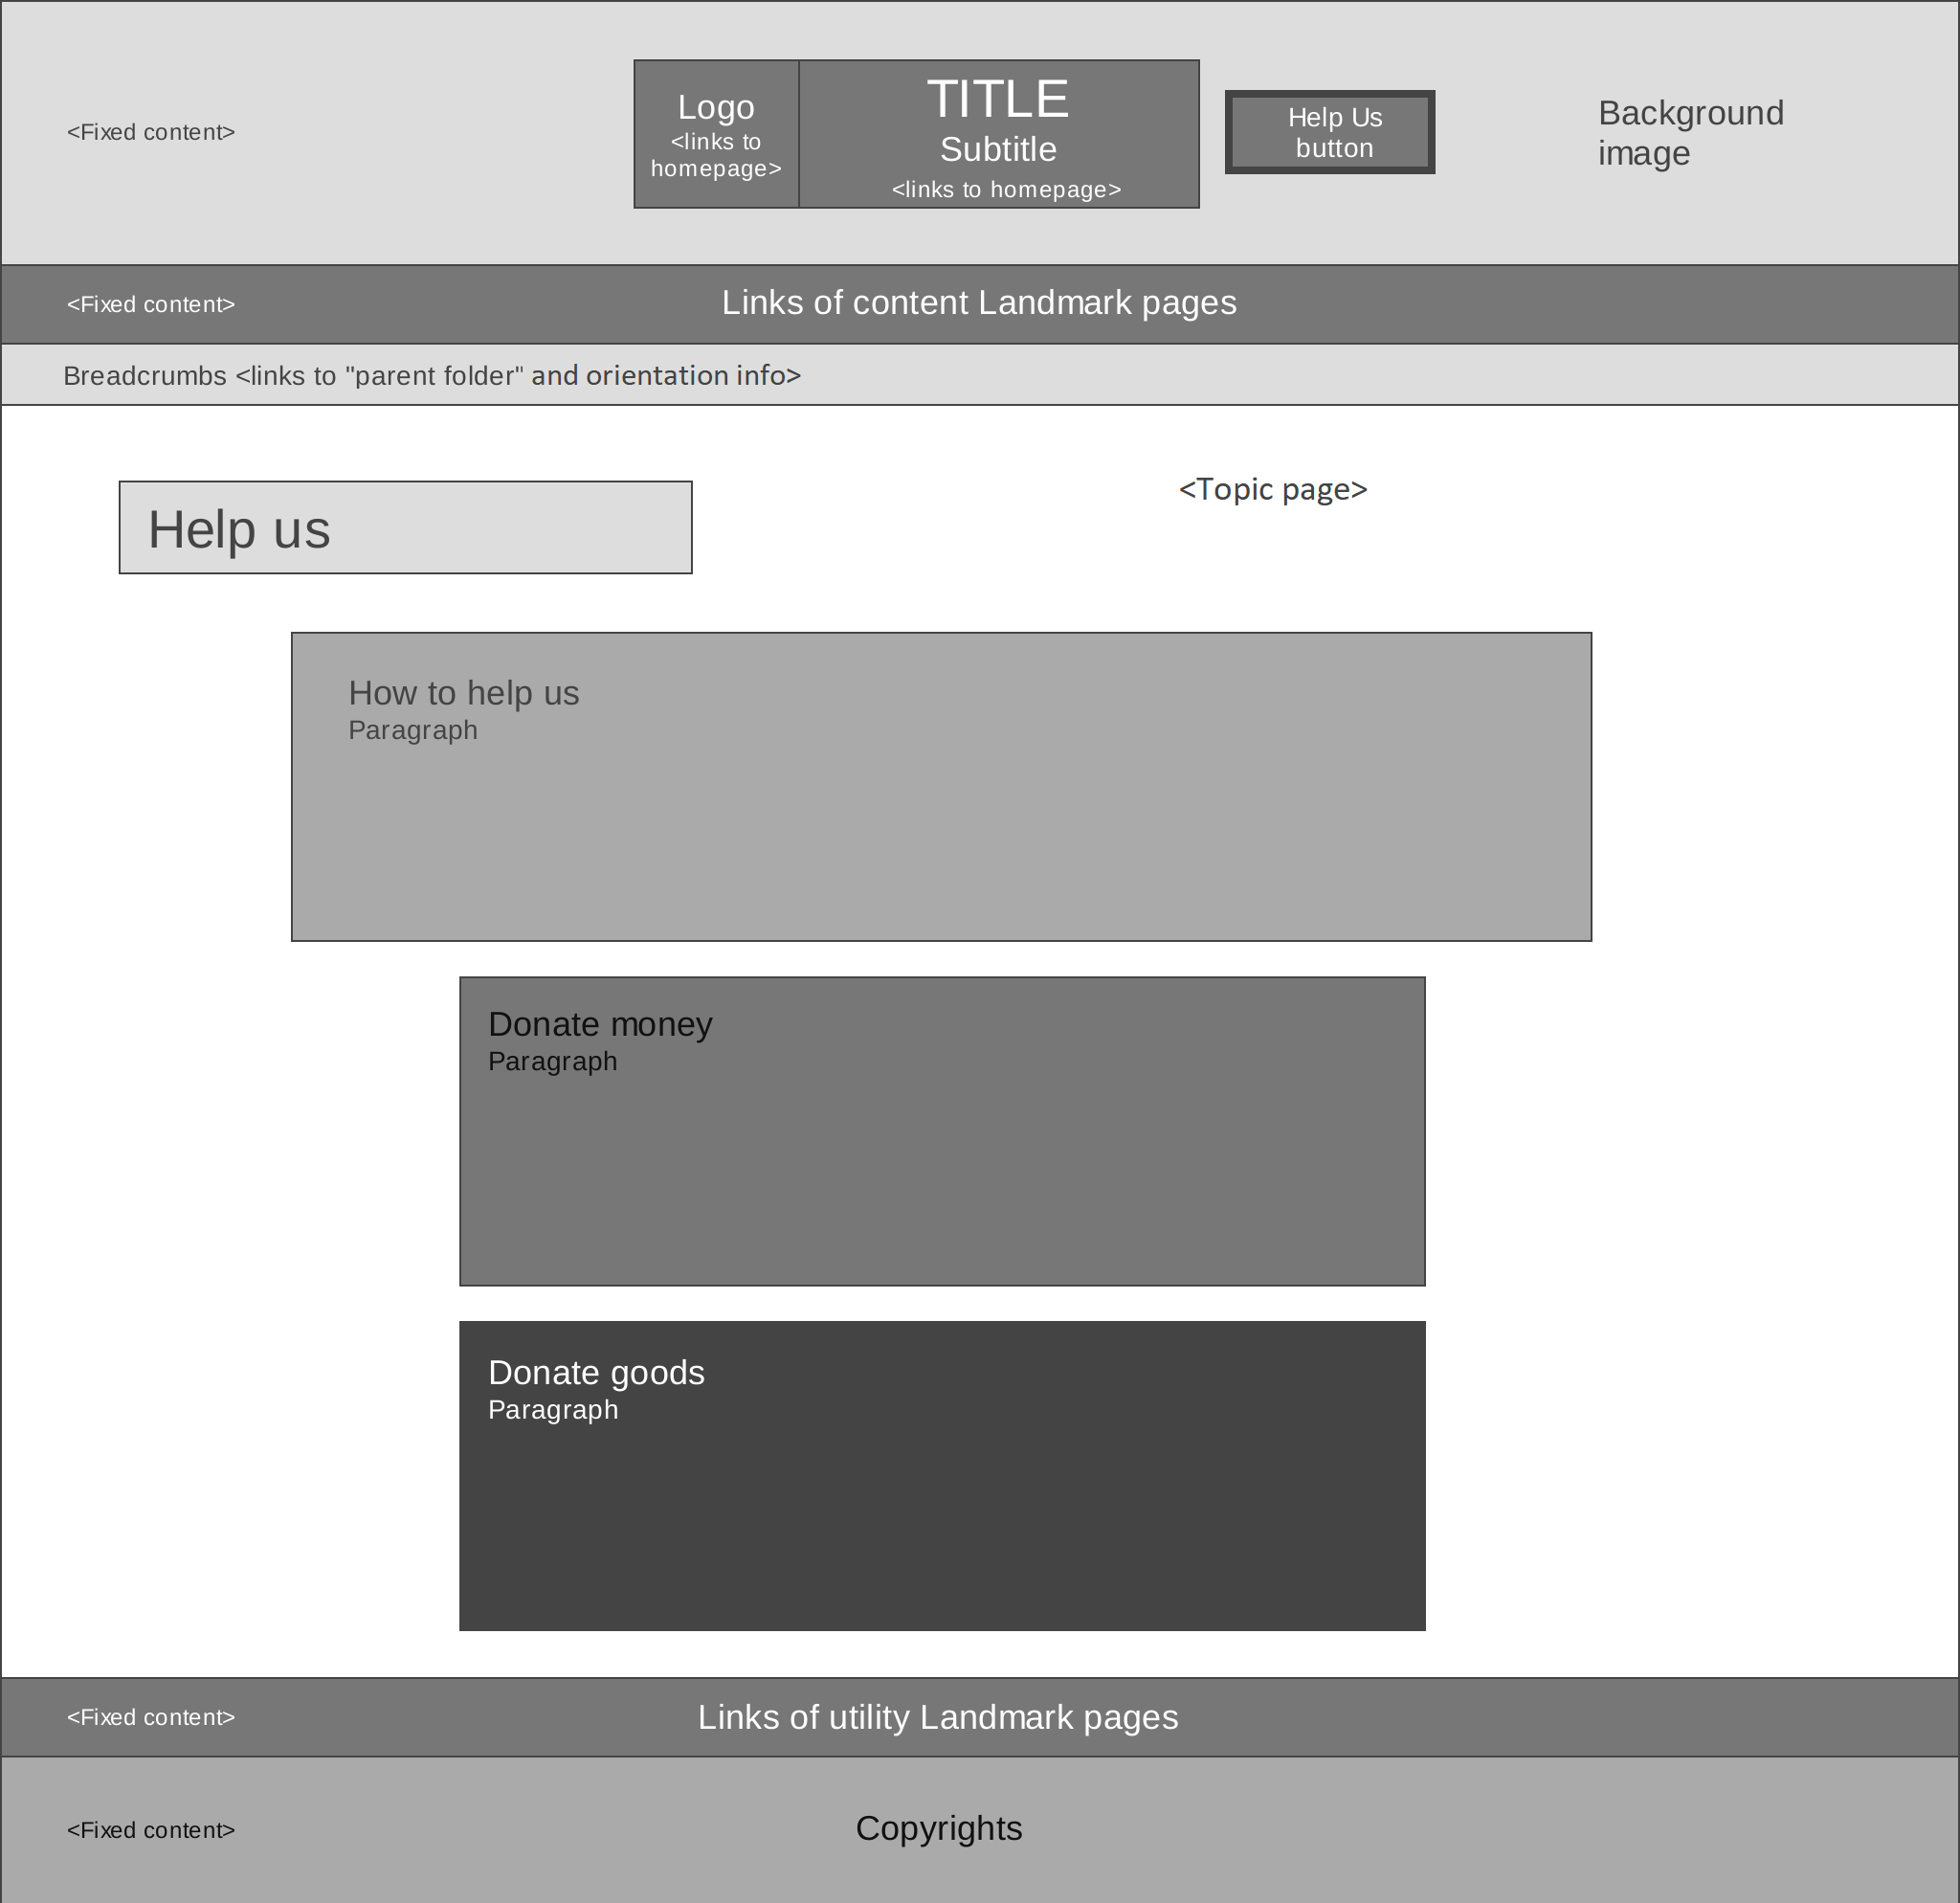
\includegraphics[width=1.3\textwidth, center]{MainMatter/images/10-Single-topic-help-us}
\caption{Single Topic Page: Help us}
\label{fig:figure2}
\end{figure}
%
%
% -----------------------------END------------------------------------- %
